\documentclass[10pt,a4paper]{article}
\usepackage[utf8]{inputenc}
\usepackage[T1]{fontenc}
\usepackage{lmodern}
\usepackage[margin=1.5cm, top=1.4cm, bottom=1.4cm]{geometry}
\usepackage{hyperref}
\usepackage{enumitem}
\usepackage{titlesec}
\usepackage{xcolor}
\usepackage{graphicx}

\definecolor{accent}{HTML}{00686E}
\hypersetup{colorlinks=true, urlcolor=accent, linkcolor=accent}
\pagenumbering{arabic}
\setlength{\parindent}{0pt}

\titleformat{\section}{\large\bfseries\color{accent}}{}{0em}{}[\vspace{-0.6em}\rule{\textwidth}{0.8pt}]
\titlespacing{\section}{0pt}{7pt}{4pt}

\newcommand{\role}[4]{%
  \textbf{#1} \hfill \textbf{#2}\\[1pt]%
  \textit{#3} \hfill \textit{#4}\\[2pt]%
}
\setlist[itemize]{leftmargin=1.2em, itemsep=1.5pt, topsep=2pt, parsep=0pt}

\begin{document}

% ================= HEADER =================
\begin{minipage}[c]{0.80\textwidth}
  {\Huge\bfseries Prabhavit Gupta}\\[3pt]
  {\color{accent}\large Senior Fullstack Developer: Claude Code, TypeScript, Node.js \& Cloud Architectures}\\[6pt]
  {\footnotesize +39 351 610 7807 ~$\vert$~
  \href{mailto:prabhavitg@gmail.com}{prabhavitg@gmail.com} ~$\vert$~
  \href{https://www.linkedin.com/in/prabhavit/}{linkedin.com/in/prabhavit} ~$\vert$~
  \href{https://github.com/prab-gupta}{github.com/prab-gupta} ~$\vert$~
  Venice, Italy (CET Time Zone / EU Permanent Resident)}
\end{minipage}\hfill
\begin{minipage}[c]{0.18\textwidth}
  \raggedleft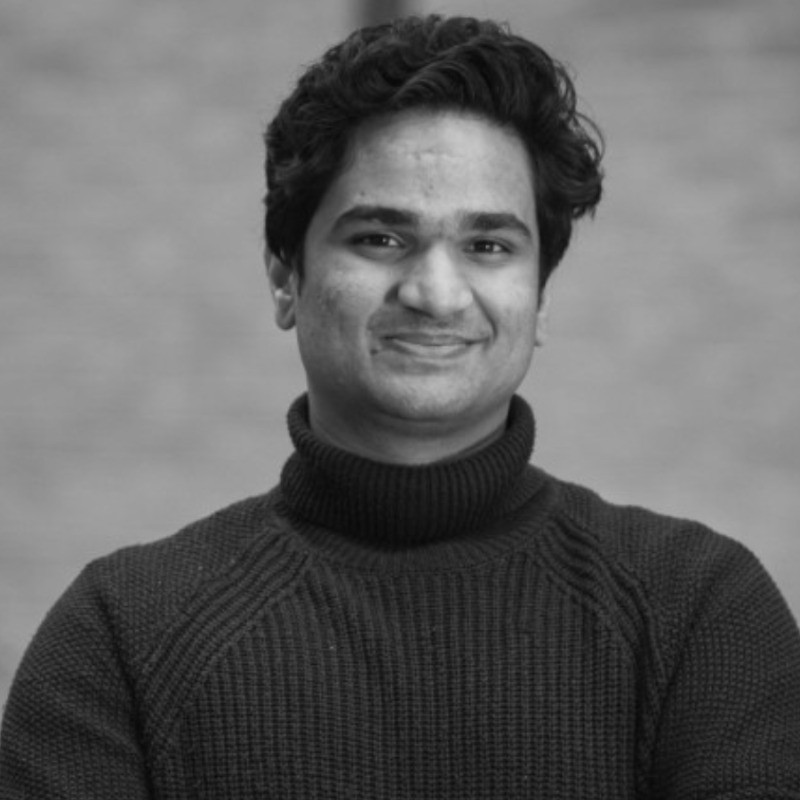
\includegraphics[width=2.0cm]{photo.jpg}
\end{minipage}
\vspace{-2pt}

% ================= SUMMARY =================
\section{Summary}
Senior Fullstack Developer and Claude Code power user with 3 years of commercial production engineering experience delivering scalable cloud backends and responsive web applications. Expert in leveraging Claude Code and agentic workflows to accelerate greenfield feature development, automate regression testing, and maintain rigorous code quality. Deep practical expertise across TypeScript, Node.js/Express, RESTful API design, OAuth2/JWT authentication, and webhook-driven cloud architectures (Stripe, Twilio, Firebase/GCP). Based in Venice, Italy (CET time zone) with an EU Long-Term Residence Permit (permanent unrestricted EU work authorization, no sponsorship needed); immediately available for remote full-time positions.

% ================= TECHNICAL EXPERTISE =================
\section{Technical Expertise}
\begin{itemize}
  \item \textbf{AI-Accelerated Engineering (Claude Code):} Advanced daily practitioner of Claude Code, MCP (Model Context Protocol), prompt engineering, and agentic tool-use pipelines for rapid feature prototyping, automated refactoring, and test synthesis.
  \item \textbf{Backend \& Cloud Services:} TypeScript (advanced), Node.js, Express, REST API design (strict HTTP status codes, error handling, validation), Firebase (Auth, Firestore, Cloud Functions, Admin SDK), GCP IAM, OAuth2 JWT token lifecycle.
  \item \textbf{Third-Party \& Webhook Integrations:} Stripe payment gateways, subscription lifecycles, Twilio communications API, webhook-driven event architectures, idempotency handling, transactional email (Mailjet/SendGrid).
  \item \textbf{Frontend \& UI Engineering:} Modern component architectures (SvelteKit, React, Next.js), TypeScript, Tailwind CSS, responsive mobile-first design, frontend state management.
  \item \textbf{DevOps \& Data Infrastructure:} GitHub Actions CI/CD pipelines for cloud functions and staging/production deployments, PostgreSQL, Redis, Docker containerization.
  \item \textbf{Languages \& Authorization:} English (C1 Professional, fluent), Hindi (Native), Italian (Conversational). EU Long-Term Residence Permit (unrestricted EU work authorization across all EU member states, no sponsorship required).
\end{itemize}

% ================= EXPERIENCE =================
\section{Experience}

\role{\href{https://flowspace.co}{FlowSpace.co}}{Mar 2024 - Aug 2026}{Full-Stack AI Engineer}{London, UK (remote)}
\begin{itemize}
  \item Spearheaded development of full-stack AI platform features using Claude Code and agentic tooling, scaling services to support 4,500+ active enterprise users with 99.8\% production uptime.
  \item Engineered high-performance backend microservices in Node.js and TypeScript, designing secure REST APIs, webhook handlers, and token-based OAuth2 authentication flows.
  \item Implemented complex Stripe billing integrations and webhook event listeners to manage customer subscription lifecycles, automated invoicing, and transaction status reconciliation.
  \item Built automated GitHub Actions CI/CD pipelines deploying cloud functions across staging and production environments, enforcing linting, type-checking, and unit test suites.
  \item Created dynamic frontend interfaces with modern reactive components, Tailwind CSS, and TypeScript, optimizing client-side performance and accessibility.
\end{itemize}

\role{Urlink}{Apr 2025 - Jul 2025}{Full-Stack Solutions Developer (Freelance)}{Barcelona, Spain (remote)}
\begin{itemize}
  \item Built responsive web applications and third-party API integration services connecting external communication channels and transactional notification systems.
  \item Designed RESTful endpoints with input validation and centralized error handling, ensuring reliable telemetry and operational logging.
  \item Configured automated GitHub workflows and environment staging configurations to streamline team releases and prevent regression.
\end{itemize}

\role{Independent Technical Consultant}{Aug 2023 - Feb 2024}{Full-Stack \& Automation Developer}{Venice, Italy}
\begin{itemize}
  \item Developed custom web platforms, automated webhook processors, and cloud integration microservices using TypeScript, Node.js, and Python for European SMB clients.
  \item Integrated automated payment and notification flows using Stripe and messaging APIs, eliminating manual billing reconciliation for non-technical stakeholders.
  \item Documented end-to-end API specifications, schema definitions, and system architecture diagrams for client maintainers.
\end{itemize}

% ================= EDUCATION =================
\section{Education}
\role{Ca' Foscari University of Venice}{2020 - 2024}{BA in Philosophy, International Studies and Economics}{Venice, Italy}
\begin{itemize}
  \item Rigorous foundational study in formal logic, epistemology, analytical problem decomposition, and systems thinking.
\end{itemize}

\end{document}
